\section{DESIGN OVERVIEW}
\subsection{EMF - Open Architecture Ware 5}
The component code generator for Alma Common Software initially created before,
was supported on Open Architecture Ware 4, since is a requirement have the
code generator based on Open Architecture Ware 5, the previous work was
migrated to oaW 5, this means that the code generator is based now on Eclipse
Modeling Framework (EMF), mainly in Xtend and Xpand subprojects.\\
\\
EMF supports many types of models like Ecore (EMF native models), UML2 models,
or, in this case meta-metamodels in XMI2.0 format. Actually the generator
support a XMI2.0 meta-metamodels, mostly of this models are created and exported
from MagicDraw UML Diagram Tool, MagicDraw generate the necessary XMI files
for later generate the code components to be implemented by the final user. 
Is important to specify that the models needs a profile file, which defines the
stereotypes for use in the generator, where they differentiate the
many characteristics or custom features in the UML model.

\subsubsection{Stereotypes}
In UML models, the use of stereotypes helps to distinguish the classes that
must be generated and how must be generated. This stereotypes are defined in
the UML profile file, which is created when the UML model is exported from
MagicDraw.\\
One of each classes may have a stereotype defined to know how the code must be
generated or specify a certain feature desired, i.e.: 

\begin{figure*}[h!t]
\begin{center}
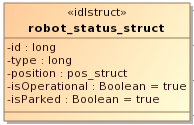
\includegraphics[scale=0.3]{images/idlstruct}
\caption{\label{fig:ex_diag}Example class with a stereotype to be generated as
a IDL struct}
\end{center}
\end{figure*}

The class  \verb robot_status_struct  has the \verb+<<IDLStruct>>+ stereotype,
then the generator call the IDLStruct template and generate the code of an IDL
file of ACS and implement such struct in the IDL file..\\
\\
There exist three main categories of stereotypes:
\begin{itemize}
	\item Class stereotype : applies to classes.
	stereotype.
	\item Property stereotype : applies to class level variables. 
	\item Operation stereotype : applies to a class method.
\end{itemize}

The stereotypes helps to differentiate how should the code must be
generated. Currently the generator has several types of (only class level)
stereotypes defined below:
\\
\begin{itemize}
	\item \verb+<<enumeration>>+: UML class is implemented as an enumeration
	and is generated in a common IDL file.
	\item \verb+<<idlstruct>>+: UML class is implemented as an IDL struct generated
	in a common IDL file.
	\item \verb+<<characteristic>>+: The UML class is implemented as a
	Characteristic Component of ACS.
	\item \verb+<<override>>+: If the UML  class is inherited, the generator
	overrides the parent methods (of the UML model) in the actual class, this only
	is applied to Java classes and not to the IDL interfaces and is implemented
	as a ACS component.
	\item \verb+<<alloverride>>+: Same as the override stereotype, if the class has
	a multi-inherited-level, the generator overrides all methods inherited in all levels in the UML model and is implemented
	as a ACS component, this only is applied to Java classes and not to the IDL interfaces.
	\item \verb+<<container>>+: The UML  class is defined as a ACS container,
	the generator reads a property called `language` to know the languageof the
	container (i.e.: language = java) and generate the necessary code to implement
	this container.
	\item \verb+<<ncconfig>>+: If the UML class has this stereotype, the
	generator reads the channels to implement (properties in the UML class) in the
	code, this channels are defined in the common IDL file of the code generated.
	\item \verb+<<ncsupplier>>+: The UML class is implemented as a ACS component
	event supplier and use a common channel that has the same name of the project.
	\item \verb+<<ncconsumer>>+: The UML class is implemented as a ACS component
	event consumer and use a common channel that has the same name of the project.
	\item \verb+<<nchybrid>>+: The UML class is implemented as a ACS component
	event supplier-consumer and use a common channel that has the same name of the
	project.
	\item \verb+<<void>>+: If this stereotype is implemented, the generator will 
	void generate the class.
\end{itemize}

The stereotypes above, are defined in the profile file of the XMI
exported UML model and can be mixed in the UML model, i.e: a class can have the 
\verb+<<ncconsumer>>+ and  \verb+<<override>>+ to generate an ACS component that
override his parent methods and is implemented as a consumer, but, not all
stereotypes can be mixed, the developer must have a certain common logic to mix
the stereotypes, this logic is related to the knowing of ACS component
development.
\\
\\
\\
\\
\\
\\
\\
Below, a table of how can mix the stereotypes:
\\
\begin {small} 
\begin{center}
\normalsize
\vskip 0.1 cm
 \begin{tabular}{| l | l | l | l | l | l | l | l | l | l | l |}
    \hline
  & \scriptsize idlstruct & \scriptsize characteristic & \scriptsize override & \scriptsize alloverride & \scriptsize container & \scriptsize ncconfig & \scriptsize ncsupplier & \scriptsize ncconsumer & \scriptsize nchybrid \\ \hline
 \scriptsize idlstruct & - &  &  & &  &  &  &  & \\ \hline 
 \scriptsize characteristic & &- & \scriptsize yes & \scriptsize yes & & & \scriptsize yes & \scriptsize yes & \scriptsize yes\\ \hline
 \scriptsize override & & \scriptsize yes &- & & & & \scriptsize yes & \scriptsize yes& \scriptsize yes\\ \hline 
 \scriptsize alloverride & & \scriptsize yes & &- & & &\scriptsize yes &\scriptsize yes &\scriptsize yes\\ \hline 
 \scriptsize container & & & & & -& & & &\\ \hline 
 \scriptsize ncconfig & & & & & & -& & &\\ \hline 
 \scriptsize ncsupplier & &\scriptsize yes &\scriptsize yes &\scriptsize yes & & &- & &\\ \hline 
 \scriptsize ncconsumer & &\scriptsize yes &\scriptsize yes &\scriptsize yes & & & &- &\\ \hline 
 \scriptsize nchybrid & &\scriptsize yes &\scriptsize yes &\scriptsize yes & & & & &-\\ \hline
\end{tabular}
\end{center}
\end{small}
\normalsize

\subsubsection{Xtend/Xpand}
Since owA was migrated to EMF, the code generator is based on a mixture of EMF
subprojects(Xpand/Xtend/Xtext) , the EMF subprojects which are used:

\begin{itemize}
	\item Xtend : provides the possibility to define rich libraries of independent
	operations and non-invasive metamodel extensions based on either Java methods
	or oAW expressions. Those libraries can be referenced from all other textual
	languages, that are based on the expressions framework, in this case Xpand.
	\item Xpand : A programming language which allow to define the templates of
	the generator and controll the output generation.
\end{itemize}

\subsubsection{Workflow File Configuration}
The workflow, is a EMF XML configuration file that controll the workflow of the
generator, in which, where configured the paths of UML exported models,
output folder, templates used, Java code beautifiers and the package name
definition for the generated code.\\
\\
The path of the model to generate, the generated code output folder path and
the UML profile file path are specified using dynamic workflow propertys by
\$\{myVariable\} sintax. These properties can be configured dynamically in the
Java program (using String Hashmap) that call the generator, or by command
line.\\
\\
Also the templates to use in the generation are specified in the configuration
file as 'Workflow Components'.\\
\\
The components must have defined :
\begin{itemize}
	\item Output path : the output path for the generated file, this is specified
	by a global property in the workflow configuration as \$\{ouputFolderURI\} 
	property.
	\item UML profile : this is specified by a global property in the workflow
	configuration as \$\{profileFileURI\} property, the generator only support
	maximum three profile files.
	\item Template : the template to use.
	\item Beautifiers : XML or Java code beautifiers.
	\item VetoStrategy : only is specified if the component will use a Veto
	Strategy, see 'Generator Optimization' section for more info about this.
	\item File encoding : by default UTF-8.
\end{itemize}

An example configuration for a component, in this case a java class files
component generator :
\begin{center}
\begin{verbatim}
    <component id="genjava" class="org.eclipse.xpand2.Generator"
     skipOnErrors="true"> 
    <fileEncoding value="UTF-8" />
        <metaModel idRef="default_profile"/>
        <expand value="templates::java::JavaRoot::Root FOR model"/>
        <outlet path="${ouputFolderURI}">
            <vetoStrategy
             class="cl.alma.acs.ccg.vetostrategy.ACSCCGVetoStrategy" /> 
            <postprocessor 
             class="org.eclipse.xpand2.output.JavaBeautifier"/>
        </outlet>
        <prSrcPaths value="${ouputFolderURI}"/>
    </component> 
\end{verbatim}
\end{center}

In the project, exists three workflow files, a Java, C++ and Python. Python
and C++ workflow files are ready to be implemented, only Java workflow is full
implemented for the generator.\\
\\
The workflow file is based in oaW 5, this means that the file presents many
changes from his previous version.

\subsubsection{Template Files}
Template files controll the output code generation. Each class in the UML model
is analyzed by the template file, the template check the stereotype of the
class and generate the output file. The templates are based in the Xpand
programming language [4].\\
All templates are encoded in UTF-8 by the use of 'guillimets' [4].

\subsubsection{Xtend Util Helper}
In the generator templates folder exists a Xtend file, this file is a helper
for the templates files, in which, are defined helper functions like if a class
is inherited from other class. More info about the functions, see 'Quick
Reference User Manual' in this document.


\subsection{Generator Optimization}
With a simple model (20 classes) the generator can take about 8 or 10 seconds
to generate the code in a Dual CPU@1.73GHz with 2048 MB RAM, but, if the model
is more complex, then the generation can take longer, this is no problem at
all, the problem comes when the code must be generated again for any
reason, like add a method in a class or add another class in the model. This is
a problem, because, every time we want re-generate the code, will take the same
time as the first generation even if there are no changes in the model (same
code to generate.)\\
\\
To fix this, the use of EMF Veto Strategy is implemented in the components
workflow file configuration. This strategy is class that implements a EMF Veto
interface class, in which each file to be generated, is analyzed if presents any
changes, if there any changes, the files is generated again, if not, the file
is not generated again.\\
\\
This strategy improves the generation time in regeneration, complex models,
and model refactoring.

\subsection{Source Code Structure}
The generator is packaged in a JAR Java file, under the reverse domain name
cl.alma.acs.ccg which follow the Java package folder structure, the source code
use Ant or Eclipse Ant to compile the project.

\begin{verbatim}
cl.alma.acs.ccg
|-- bin
|   |-- ACSCCG.class
|   |-- cl
|   |   `-- alma
|   |       `-- acs
|   |           `-- ccg
|   |               |-- mwe
|   |               |   |-- CppWorkflow.mwe
|   |               |   |-- JavaWorkflow.mwe
|   |               |   `-- PythonWorkflow.mwe
|   |               |-- strategy
|   |               |   |-- CodeCppGeneration.class
|   |               |   |-- CodeJavaGeneration.class
|   |               |   |-- CodePythonGeneration.class
|   |               |   |-- ContextCodeGeneration.class
|   |               |   `-- ICodeGenerationStrategy.class
|   |               |-- vetostrategy
|   |               |   `-- ACSCCGVetoStrategy.class
|   |               `-- vo
|   |                   `-- VOGenerator.class
|   `-- templates
|       |-- cpp
|       |-- java
|       |   |-- CDB.xpt
|       |   |-- IDLCommonRoot.xpt
|       |   |-- IDLCommon.xpt
|       |   |-- IDLComponent.xpt
|       |   |-- JavaCharacteristicComponent.xpt
|       |   |-- JavaComponent.xpt
|       |   |-- JavaContainer.xpt
|       |   |-- JavaHelper.xpt
|       |   |-- JavaInheritanceAllOverride.xpt
|       |   |-- JavaInheritanceOverride.xpt
|       |   |-- JavaInterfaceImplements.xpt
|       |   |-- JavaInterface.xpt
|       |   |-- JavaRoot.xpt
|       |   |-- Makefile.xpt
|       |   |-- SchemaRoot.xpt
|       |   |-- Schema.xpt
|       |   `-- xJavaUtil.ext
|       `-- python
|-- build.properties
|-- build.xml
|-- lib
|   `-- commons-cli-1.2.jar
|-- META-INF
|   `-- MANIFEST.MF
|-- project
`-- src
    |-- ACSCCG.java
    |-- cl
    |   `-- alma
    |       `-- acs
    |           `-- ccg
    |               |-- mwe
    |               |   |-- CppWorkflow.mwe
    |               |   |-- JavaWorkflow.mwe
    |               |   `-- PythonWorkflow.mwe
    |               |-- strategy
    |               |   |-- CodeCppGeneration.java
    |               |   |-- CodeJavaGeneration.java
    |               |   |-- CodePythonGeneration.java
    |               |   |-- ContextCodeGeneration.java
    |               |   `-- ICodeGenerationStrategy.java
    |               |-- vetostrategy
    |               |   `-- ACSCCGVetoStrategy.java
    |               `-- vo
    |                   `-- VOGenerator.java
    `-- templates
        |-- cpp
        |-- java
        |   |-- CDB.xpt
        |   |-- IDLCommonRoot.xpt
        |   |-- IDLCommon.xpt
        |   |-- IDLComponent.xpt
        |   |-- JavaCharacteristicComponent.xpt
        |   |-- JavaComponent.xpt
        |   |-- JavaContainer.xpt
        |   |-- JavaHelper.xpt
        |   |-- JavaInheritanceAllOverride.xpt
        |   |-- JavaInheritanceOverride.xpt
        |   |-- JavaInterfaceImplements.xpt
        |   |-- JavaInterface.xpt
        |   |-- JavaRoot.xpt
        |   |-- Makefile.xpt
        |   |-- SchemaRoot.xpt
        |   |-- Schema.xpt
        |   `-- xJavaUtil.ext
        `-- python
\end{verbatim}

\newpage

\subsubsection{Class Diagram}
In the class diagram, the only classes not developed (in the project) are those
which belongs to the packages {\tt org.eclipse.xpand2.output}  and {\tt
org.eclipse.emf.mew.core}.\\ 
\begin{figure*}[h!t]
\begin{center}
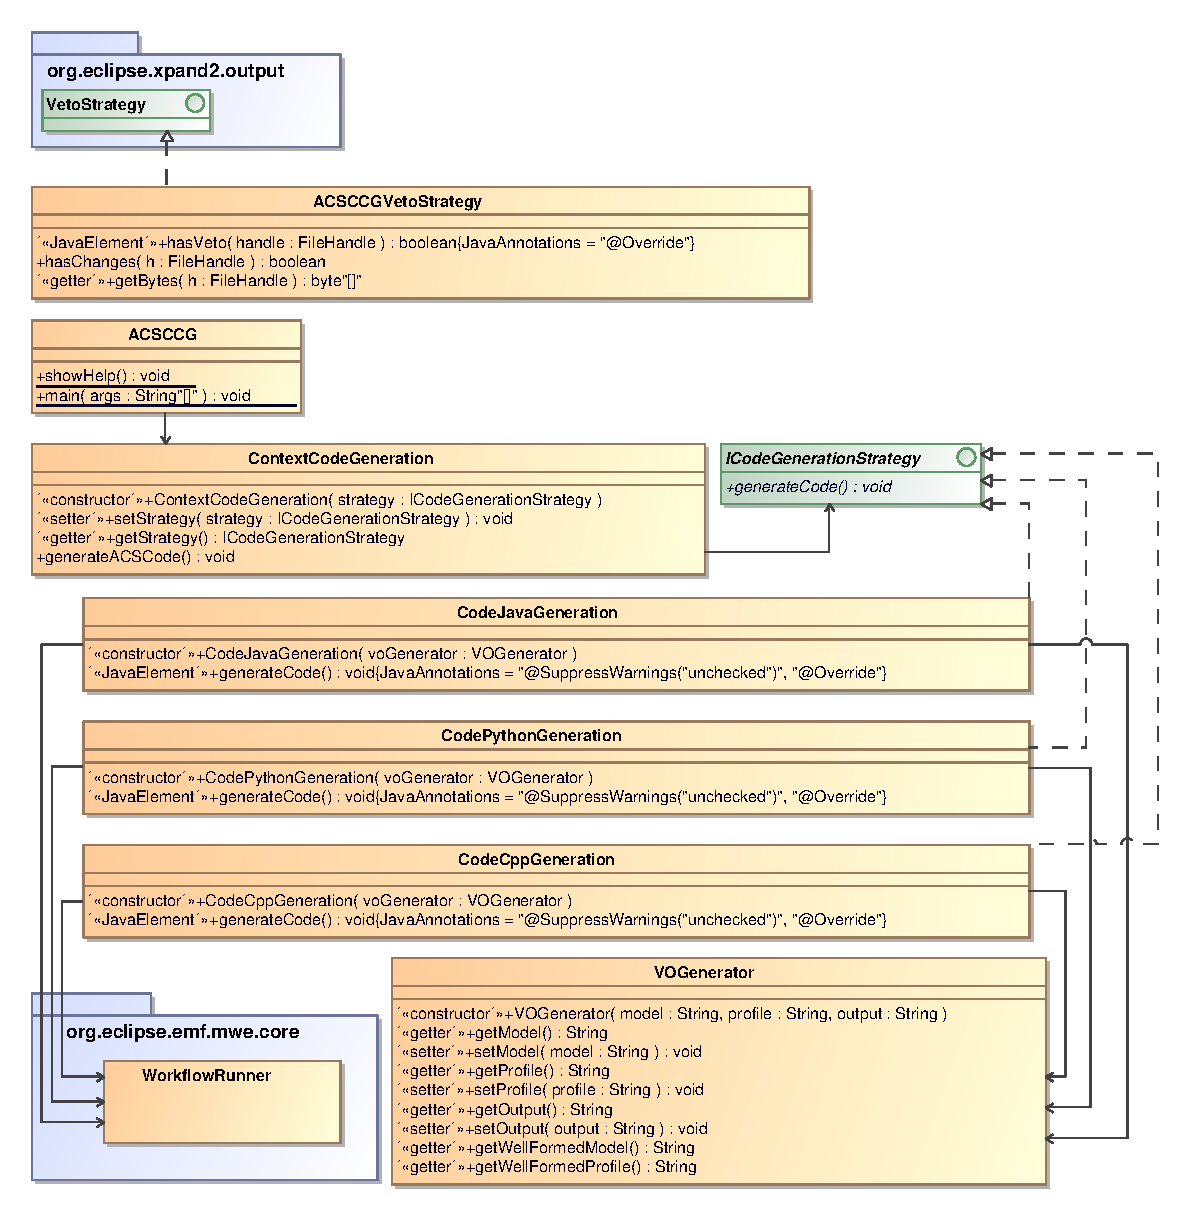
\includegraphics[scale=0.85]{images/ccgclassdiagram}
\caption{\label{fig:main_diag}Component Code Generator Class Diagram}
\end{center}
\end{figure*}

\newpage

\subsubsubsection{Strategy Pattern}
A Strategy Pattern (Policy Pattern) was implemented in the component code
generator to generate the code for each programming languaje in ACS whithout
change top levels algorithms, due to the scope of the project, only Java
strategy is full implemented. 
\begin{figure*}[h!t]
\begin{center}
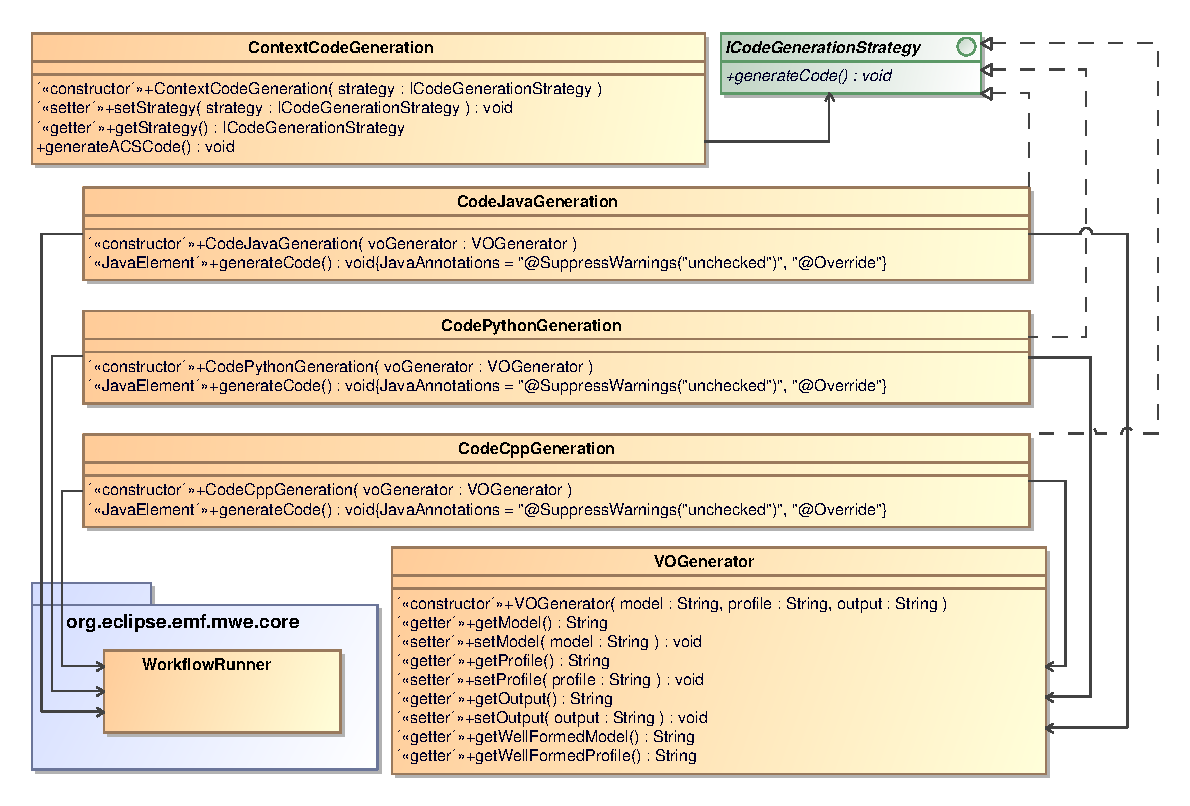
\includegraphics[scale=0.85]{images/strategypattern}
\caption{\label{fig:sp_diag}Strategy Pattern}
\end{center}
\end{figure*}
\\The {\tt ContextCodeGeneration} is the main class to be called for implement
the generator in plugins, Java programs or other enviroments.

\newpage

\subsubsubsection{EMF Veto Strategy}
The class {\tt ACSCCGVetoStrategy} is called by WorkflowRunner in runtime of
the component code generator, for more info about Veto, see Generator
Optimization section in this document. 
\begin{figure*}[h!t]
\begin{center}
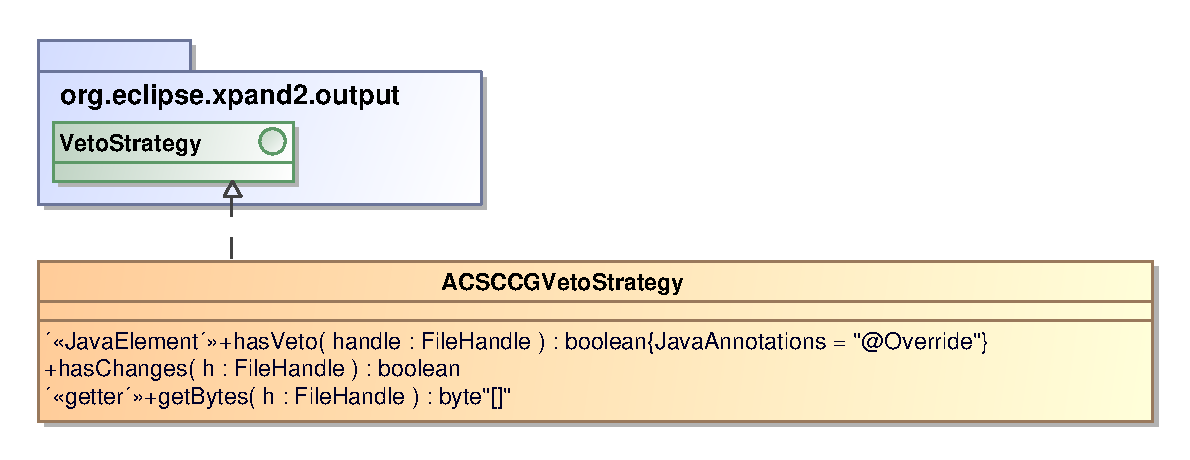
\includegraphics[scale=0.65]{images/vetostrategy}
\caption{\label{fig:vs_diag}EMF Veto Strategy}
\end{center}
\end{figure*}
%\begin{center}
%TABLE OF TIMES
%\end{center}

%\newpage

%\subsubsection{Sequence Diagram}
%To be implemented
%\subsubsection{Process Diagram}
%To be implemented